\documentclass{beamer}

\usepackage{graphicx}
\usepackage{hyperref}
\usepackage[latin1]{inputenc}
\usepackage[T1]{fontenc}
\usepackage[english]{babel}
\usepackage{listings}
\usepackage{xcolor,mathrsfs,url}
\usepackage{amssymb}
\usepackage{amsmath}
\usepackage{ifthen}

% The command to define a subsection is '\subsec{}' and NOT '\subsection'.
% This code generates the bar. Don't edit.
\newcommand{\midbarnew}{}
\newcommand{\subsec}[1]
{
  \ifthenelse{\equal{#1}{}}
  {\renewcommand{\midbarnew}{} \subsection{}}
  {\renewcommand{\midbarnew}{ $\mid$ } \subsection{#1}}
}

% change the pictures here, if necessary. logobig and logosmall are the internal names
% for the pictures: do not modify them, just change "hulogo" and "logo". Pictures must be 
% supplied as JPEG, PNG or PDF
%########################################

\pgfdeclareimage[height=2cm]{logobig}{logo} % use hucase instead for the Humboldt-Case Logo
\pgfdeclareimage[height=1cm]{logosmall}{logo}

% use this number to modify the scaling of the headline on titlepage
\def\titlescale{1.0}


\title{Fixed Exchange Rates}
\author{Instructor: David Jinkins\thanks{I wish to acknowledge Battista Severgnini for providing last year's slides to me. His generosity saved me much time, and these slides are partially based on his. Any errors are of course my own.}}
\date{Date: Oct. 14, 2014}
%Start of the document
\begin{document}

\frame[plain]{% create the titleslide, layout controlled in metricsbeamer
	\titlepage
}

\frame{% how to print
\frametitle{Last time}
Chapter 17:
\begin{itemize}
\item Determinants of aggregate demand in the short run
\item Short run equilibrium for aggregate demand and output (DD curve)
\item Short run equilibrium in the asset markets (AA curve)
\item Short run equilibrium (AA \& DD)
\item Temporary changes in monetary and fiscal policy
\item Permanent changes in monetary and fiscal policy
\item Odds and ends
\end{itemize}
}

\frame{% how to print
\frametitle{Plan for Today}
Chapter 18:
\begin{itemize}
\item Balance sheets of central banks
\item Fixed exchange rate
\item Monetary and fiscal policies under fixed exchange rates
\item Financial crises and capital flight
\item Interest rate differentials
\item Types of fixed exchange rate systems
\end{itemize}
Chapter 19:
\begin{itemize}
\item Goals of macroeconomic policies
\end{itemize}
}

\begin{frame}{But first a review}
\end{frame}

% \frame[plain]{\includegraphics[page=44,width=\textwidth]{ppp.pdf}}
% \frame[plain]{\includegraphics[page=47,width=\textwidth]{ppp.pdf}}
% \frame[plain]{\includegraphics[page=50,width=\textwidth]{ppp.pdf}}
% \frame[plain]{\includegraphics[page=52,width=\textwidth]{ppp.pdf}}
% \frame[plain]{\includegraphics[page=53,width=\textwidth]{ppp.pdf}}
% \frame[plain]{\includegraphics[page=54,width=\textwidth]{ppp.pdf}}
% \frame[plain]{\includegraphics[page=55,width=\textwidth]{ppp.pdf}}
% \frame[plain]{\includegraphics[page=57,width=\textwidth]{ppp.pdf}}
% \frame[plain]{\includegraphics[page=58,width=\textwidth]{ppp.pdf}}
% \frame[plain]{\includegraphics[page=60,width=\textwidth]{ppp.pdf}}
% \frame[plain]{\includegraphics[page=61,width=\textwidth]{ppp.pdf}}
% \frame[plain]{\includegraphics[page=62,width=\textwidth]{ppp.pdf}}
% \frame[plain]{\includegraphics[page=63,width=\textwidth]{ppp.pdf}}
% \frame[plain]{\includegraphics[page=65,width=\textwidth]{ppp.pdf}}
% \frame[plain]{\includegraphics[page=69,width=\textwidth]{ppp.pdf}}
% \frame[plain]{\includegraphics[page=74,width=\textwidth]{ppp.pdf}}
% \frame[plain]{\includegraphics[page=75,width=\textwidth]{ppp.pdf}}
% \frame[plain]{\includegraphics[page=76,width=\textwidth]{ppp.pdf}}
% \frame[plain]{\includegraphics[page=77,width=\textwidth]{ppp.pdf}}
% \frame[plain]{\includegraphics[page=78,width=\textwidth]{ppp.pdf}}
% \frame[plain]{\includegraphics[page=79,width=\textwidth]{ppp.pdf}}
% \frame[plain]{\includegraphics[page=80,width=\textwidth]{ppp.pdf}}
% \frame[plain]{\includegraphics[page=82,width=\textwidth]{ppp.pdf}}
% \frame[plain]{\includegraphics[page=83,width=\textwidth]{ppp.pdf}}
% \frame[plain]{\includegraphics[page=84,width=\textwidth]{ppp.pdf}}

\begin{frame}{Review}
    \begin{itemize}
        \item End review
    \end{itemize}
\end{frame}

\frame{% how to print
\frametitle{}
\begin{center}
\textcolor{blue}{Chapter 18. Fixed Exchange Rates and Foreign Exchange Intervention
}
\end{center}
}

\frame{% how to print
\frametitle{Exchange Rates}
\begin{enumerate}
\item \textbf{Fixed or Pegged} 
\item \textbf{Flexible}
\end{enumerate}
}

\frame{% how to print
\frametitle{Why Study Fixed Exchange Rates?}
\begin{enumerate}
    \item Rich, industrialized countries: The dirty float
    \item Regional currency arrangements (Denmark in the textbook!)
    \item Developing countries fix to baskets or currencies 
    \item Lessons from the history of exchange rates intervention
\end{enumerate}
Bottom line: Still a lot of intervention today
}


\frame{% how to print
\frametitle{Central Bank's Simplified Balance Sheet}
\textbf{Assets}
\begin{itemize}
\item Foreign government bonds (official international reserves)
\item Gold (official international reserves)
\item Domestic government bonds 
\item Loans to domestic banks (called discount loans in US)
\end{itemize}
\textbf{Liabilities}
\begin{itemize}
\item Deposits of domestic banks
\item Currency in circulation (previously central banks had to give up gold when citizens brought currency to exchange)
\end{itemize}
\textbf{Asset=Liabilities+ Net worth}\\
Net Worth is assumed to be zero:
\begin{center}
$\Delta Asset=\Delta Liabilities$
\end{center}
}


\frame{% how to print
\frametitle{Central Bank's Simplified Balance Sheet}
Changes in the central bank's balance sheet lead to changes in currency in circulation or changes in deposits of banks, which lead to changes in the money supply.\\
If bank deposit $\Uparrow\Rightarrow$ additional fund for customers $\Rightarrow M^{s} \Uparrow$ 
}
\frame{% how to print
\frametitle{Purchase \& Sale}
\begin{enumerate}
\item \textbf{Purchase:} central bank  buys domestic bonds or foreign bonds $\Rightarrow +\Delta Asset=+\Delta Liabilities \Rightarrow M^{s}\Uparrow$ 
\item \textbf{Sale:} central bank sells domestic bonds or foreign bonds $\Rightarrow -\Delta Asset=-\Delta Liabilities \Rightarrow M^{s}\Downarrow$ 
\end{enumerate}
\begin{itemize}
\item Foreign currency deposits and foreign government bonds are substitutes (liquidity)
\item Purchase and sale influence money supply 
\item Money supply affects the exchange rate both in the short and long-run
\end{itemize}
}

\frame{% how to print
\frametitle{Sterilization}
\begin{itemize}
    \item Suppose the central bank sells foreign currency in the foreign exchange market
    \begin{itemize}
        \item Assets decrease, liabilities decrease (why?)
        \item Money supply decreases
    \end{itemize}
    \item Suppose the central bank wants to leave money supply unchanged
    \begin{itemize}
        \item Buy domestic bonds (T-Bills, for example)
        \item Assets increase, liabilities increase
        \item Money supply returns to original level
    \end{itemize}
    \item \emph{Sterilization}: offsetting foreign asset transactions with domestic asset transactions
\end{itemize}
}

\begin{frame}{Central bank transactions}
    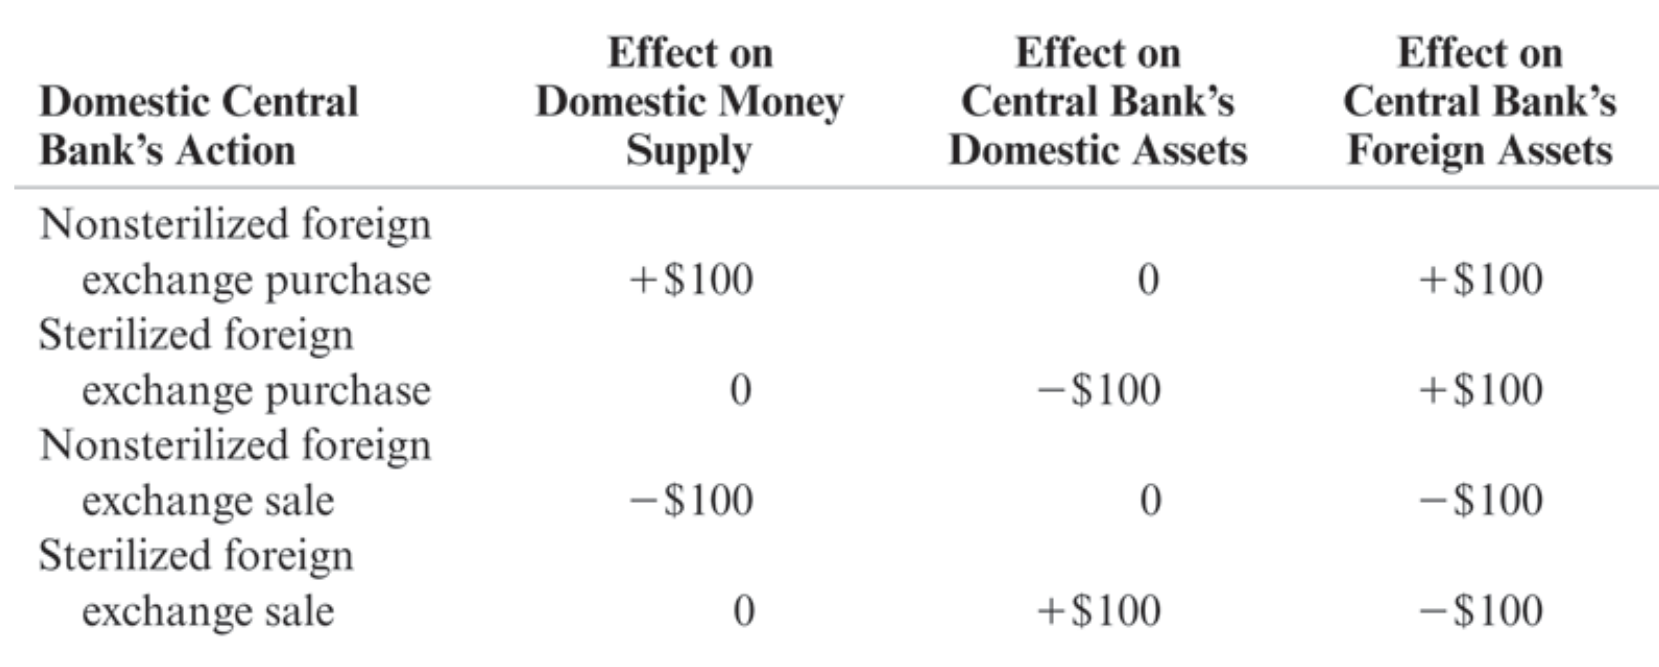
\includegraphics[scale=0.20]{central_bank_balance.png}
\end{frame}

\frame{% how to print
\frametitle{Fixed Exchange Rate}
To fix the exchange rate, a central bank influences the quantities supplied and demanded of currency by trading domestic and foreign assets, so that the exchange rate (the price of foreign currency in terms of domestic currency) stays constant.
So the UIRP 
\begin{center}
$  R = R^{*}+ \frac{\left(E^{e} -E\right)}{E}$
\end{center}
can be rewritten as
\begin{center}
$  R = R^{*}$
\end{center}
Why?
}

\frame{% how to print
\frametitle{Fixed Exchange Rate}
To fix the exchange rate, the central bank must trade foreign and domestic assets in the foreign exchange market until 
\begin{center}
$R = R^{*}$
\end{center}
or 
\begin{center}
$\frac{M^{s}}{P}=L\left(R^{*}, Y\right)$
\end{center}
Why?
}

\begin{frame}{Example}

    \begin{itemize}
        \item Level of output rises
        \item How does Central bank respond to maintain fixed exchange rate in the short run?
    \end{itemize}

\end{frame}

\frame{% how to print
\frametitle{Fixed Exchange Rate}
Assumptions:
\begin{itemize}
\item fixed exchange rate $E_{t}=E_{0}$
\item if $Y\Uparrow\Rightarrow L\left(R, Y\right) \Uparrow$
\end{itemize}
In order to maintain fixed exchange rate:
\begin{itemize}
\item Central bank buys assets denominated in foreign currency and sells domestic currency
    \begin{itemize}
        \item the price/value of foreign currency increases
        \item the price/value of domestic currency decreases
    \end{itemize}
\item This means monetary policy cannot be used for other purposes 
\item That is, the central bank no longer able to control short-run employment and output
\item As long as peg, Danes might as well adopt Euro! 
\end{itemize}
}

\frame[plain]{
\frametitle{Asset Market Equilibrium with a Fixed Exchange Rate, $E_{0}$}
\begin{figure}
	\centering
		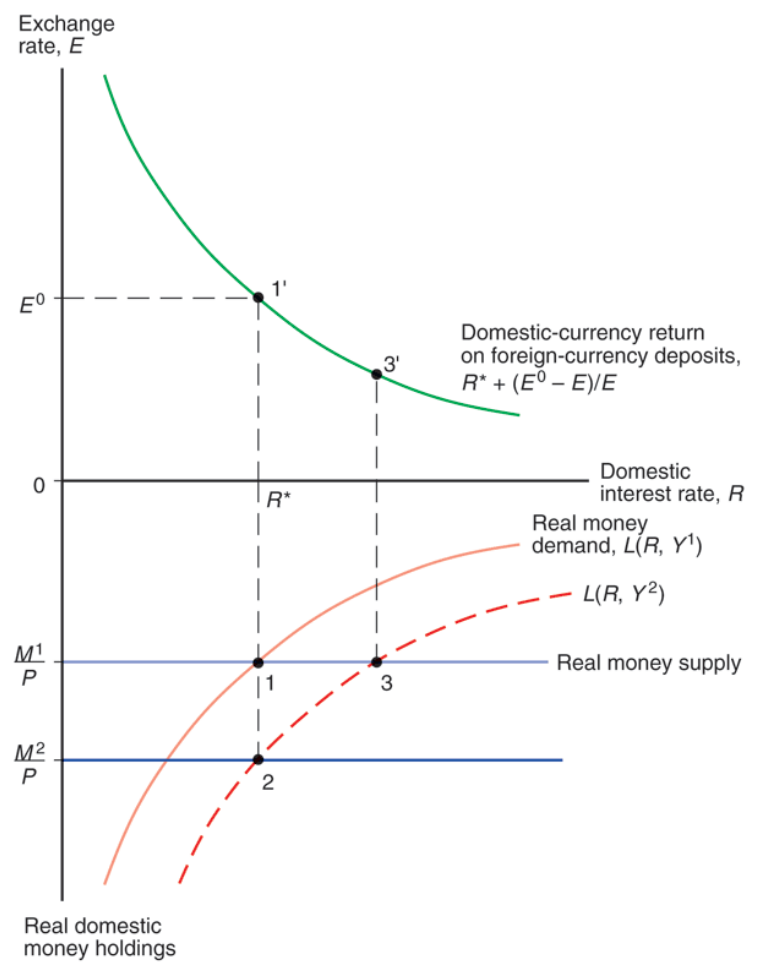
\includegraphics[scale=0.25]{foreign_exchange_control.png}
\end{figure}
}

\begin{frame}{Currency peg and monetary policy}

    \begin{itemize}
        \item Suppose as in last chapter a temporary decrease in aggregate demand
        \item Shift $DD$ curve in
        \item Last chapter: Temporary increase in money supply 
        \item Shift $AA$ curve out, maintain full employment 
        \begin{itemize}
            \item BUT: also depreciate currency!
            \item Not possible with a peg
        \end{itemize}
    \end{itemize}

\end{frame}
        
\frame[plain]{
\frametitle{Monetary Expansion Is Ineffective Under a Fixed Exchange Rate}
\begin{figure}
	\centering
		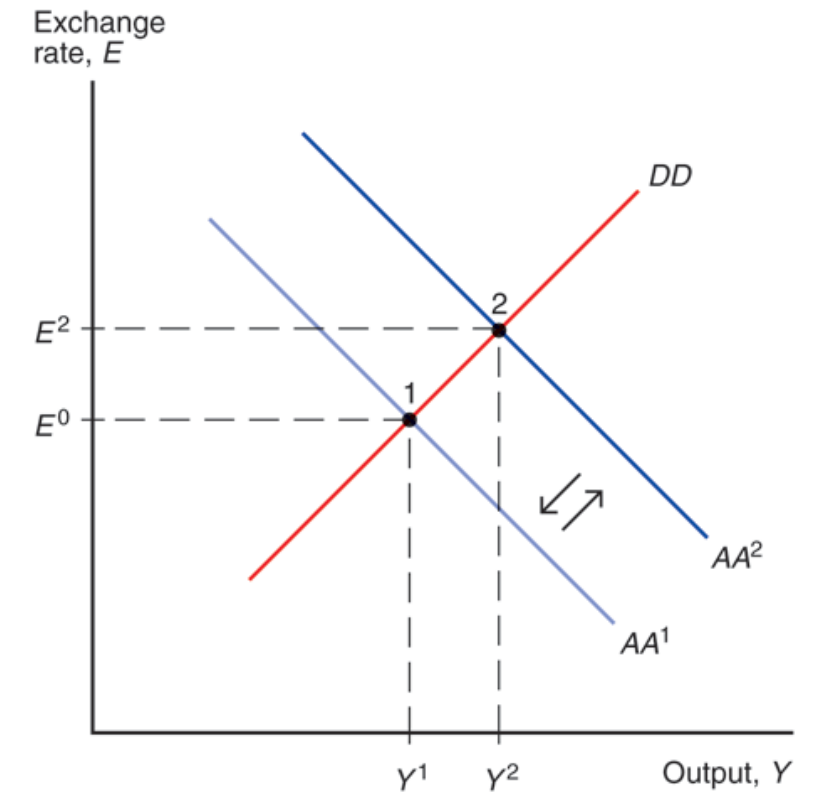
\includegraphics[scale=0.25]{ineffective_monetary.png}
\end{figure}
}



\frame{% how to print
\frametitle{Fiscal Policy and Fixed Exchange Rates in the Short Run}
On the other hand, temporary changes in fiscal policy are more effective in influencing output and employment in the short run:
\begin{center}
if $G \Uparrow$ (or $T \Downarrow$) $\Rightarrow D\Uparrow, Y\Uparrow \Rightarrow L\left(R, Y\right) \Uparrow \Rightarrow R \Uparrow \Rightarrow E \Downarrow$
\end{center}
In order to have $E_{t}=E_{0}$, central bank must buy foreign assets, thereby increasing the money supply and decreasing interest rates.
}

\frame[plain]{
\frametitle{Fiscal Expansion Under a Fixed Exchange Rate}
\begin{figure}
	\centering
		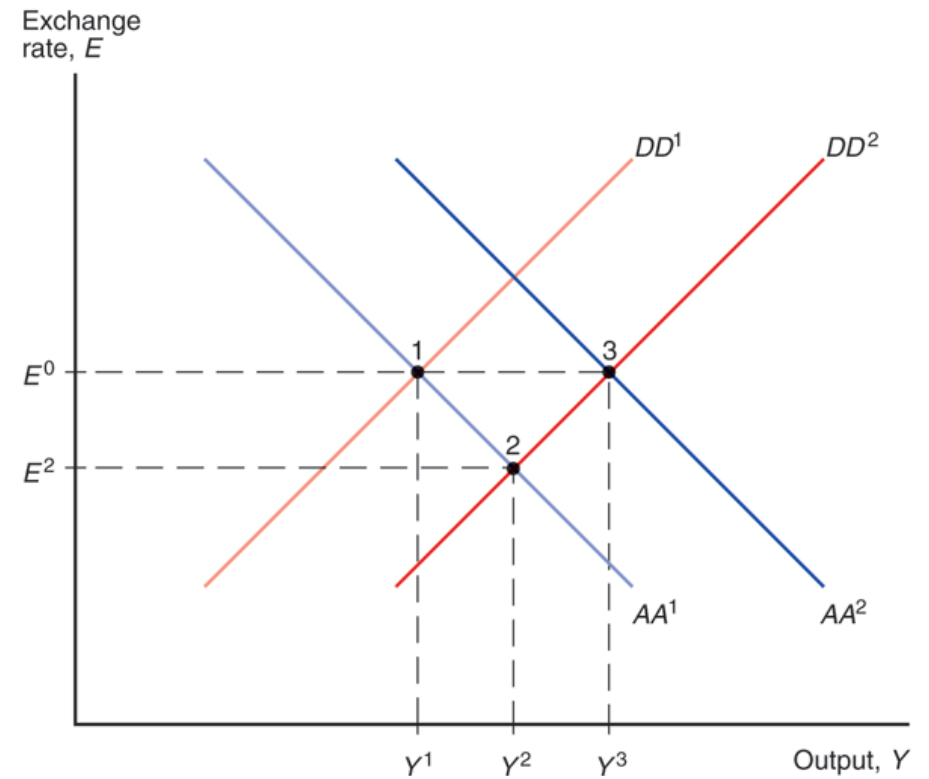
\includegraphics[scale=0.25]{fiscal_expansion_fixed.png}
\end{figure}
}
 
\frame{
\frametitle{Fiscal Policy and Fixed Exchange Rates in the Long Run}
\begin{itemize}
\item if $\frac{P^{*}}{P}\Downarrow \Rightarrow q \Downarrow \Rightarrow AD \Rightarrow$ DD curve shifts in 
\item Why does a rise in the real exchange rate cause an inward shift of aggregate demand?
\item P tends to rise until output falls to their normal (potential or natural) level.
\end{itemize}
Central bank intervenes in the foreign exchange markets:
\begin{itemize}
\item AA curve shifts in as prices rise
\item Nominal exchange rate is fixed 
\item Real exchange rate falls
\end{itemize}
$Y^f = D(E \frac{P^*}{P},Y^f-T,I,G)$
}

\begin{frame}{Pause}
    \begin{itemize}
        \item How does central bank control the exchange rate?
        \item A currency peg ties the central bank's hands
        \begin{itemize}
            \item Monetary policy no longer effective
            \item Fiscal policy becomes more effective
        \end{itemize}
        \item After an intervention, prices rise to return output to long-run level
        \item Next: Balance of payments crisis
    \end{itemize}
\end{frame}

\frame{
\frametitle{Devaluation \& Revaluation}
\begin{itemize}
\item \textbf{devaluation:} a unit of domestic currency is made less valuable, so that more units must be exchanged for 1 unit of foreign currency.
\item \textbf{revaluation:} a unit of domestic currency is made more valuable, so that fewer units need to be exchanged for 1 unit of foreign currency.
\item What do we call a change in currency value under for floating exchange rates?
\end{itemize}
}

\begin{frame}{Devaluation 101}

    \begin{itemize}
        \item Devaluation is pretty easy
        \item Central bank just announces new price of domestic currency
        \item Moment after announcement:
        \begin{itemize}
            \item Foreign currency buys more domestic currency from central bank than market
            \item People sell central bank a ton of foreign currency
            \item Market floods with domestic currency until market adjusts
            \item Central bank ends up with large foreign currency reserves
        \end{itemize}
    \end{itemize}

\end{frame}

\frame[plain]{
\frametitle{Effect of a Currency Devaluation}
\begin{figure}
	\centering
		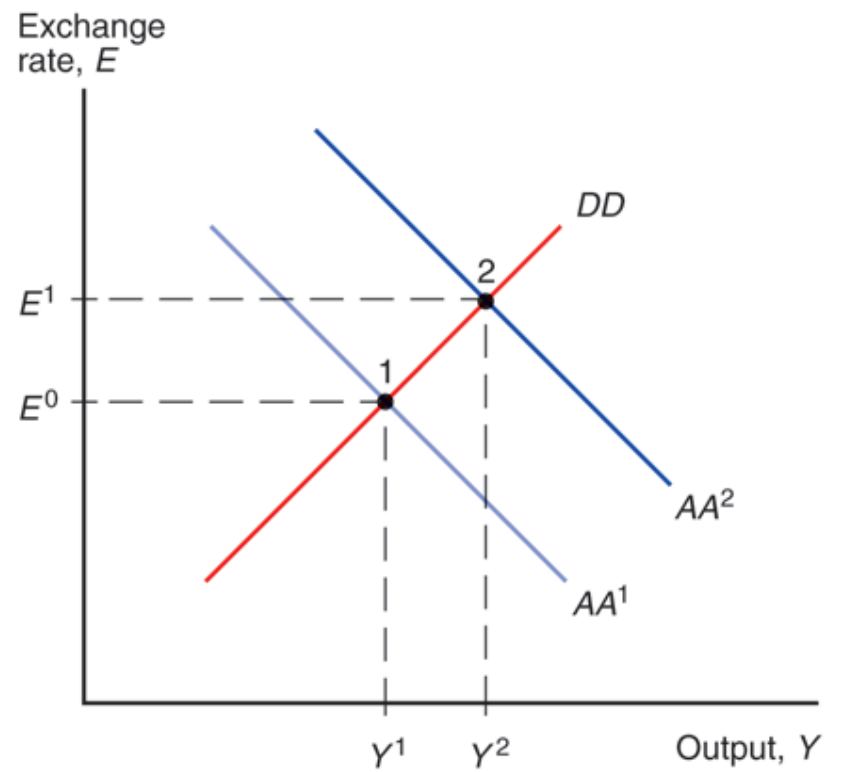
\includegraphics[scale=0.25]{devaluation.png}
\end{figure}
}

\frame{
\frametitle{Financial Crises and Capital Flight}
\textbf{Balance of payments crisis:} central bank does not have enough official foreign reserves to maintain a fixed exchange rate.
\begin{itemize}
    \item Basic recipe for BOP crises
    \begin{enumerate}
        \item Increased pressure on currency to depreciate
        \item Peg maintained by central bank selling foreign reserves
        \item People expect central bank to run out of reserves
        \item Implies future depreciation of domestic currency 
        \item Makes people want foreign assets, decreases domestic currency value
        \item Repeat
    \end{enumerate}
    \item Eventually central bank runs out of foreign reserves
\end{itemize}}

\begin{frame}{BOP Crisis}
If investors believe that the domestic currency will be devalued:
\begin{itemize}
\item Rush to sell domestic currency
\item Sell domestic assets, \emph{capital flight}
\begin{itemize}
    \item But real domestic production is ok\dots
\end{itemize}
\item central bank: $M^{s}\Downarrow \Rightarrow R\Uparrow$
\item $D \Downarrow, Y \Downarrow$ employment $\Downarrow$
\end{itemize}
\end{frame}

\frame[plain]{
\frametitle{Capital Flight, the Money Supply, and the Interest Rate}
\begin{figure}
	\centering
		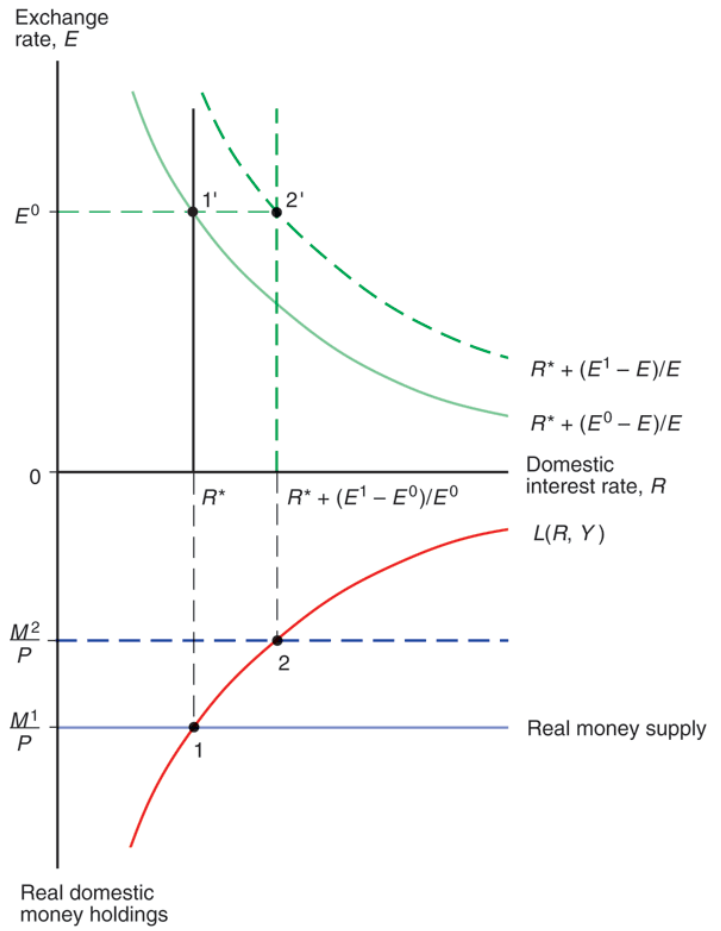
\includegraphics[scale=0.25]{money_supply_interest_attack.png}
	\label{fig:11}
\end{figure}
}

\begin{frame}{Beliefs}
\begin{itemize}
    \item Expectations of devaluation can cause a devaluation: \textbf{self-fulfilling crisis}.
    \item Modern macroeconomics is driven by belief and expectations
    \item A short history:
    \begin{enumerate}
        \item Before 1970, ad-hoc
        \item 1970's: rational expectations revolution
        \item 1980's: sunspots and weird behavior
        \item 1990's: bubbles and noise-traders 
        \item 2000's: Rational inattention
        \item Fringe: Agent-based modelling
    \end{enumerate}
    \item Recently lots of criticism, but macro chugs along
\end{itemize}
\end{frame}

\frame{
\frametitle{When Exchange Rates Misbehave}
\begin{itemize}
\item \textbf{Exchange rate crises} occur when a currency experiences a sudden change in value against another world currencies.
\begin{itemize}
\item Such crises are fairly common, 19 crises 1980-2002
\end{itemize}
\item Crises can have severe economic consequences.
\begin{itemize}
\item Government default
\item Severe changes in lending positions (bank collapse)
\item Contraction in output and decline in real wages
\end{itemize}
\item Also politically embarrassing
\begin{itemize}
\item Countries experiencing crises often seek loans from international development agencies, such as the International Monetary Fund (IMF).
\item Idea: use foreign currency to change money supply 
\end{itemize}
\end{itemize}}

\frame[plain]{
\frametitle{When Exchange Rates Misbehave. Source: IMF, International Financial Statistics.
}
\begin{figure}
	\centering
		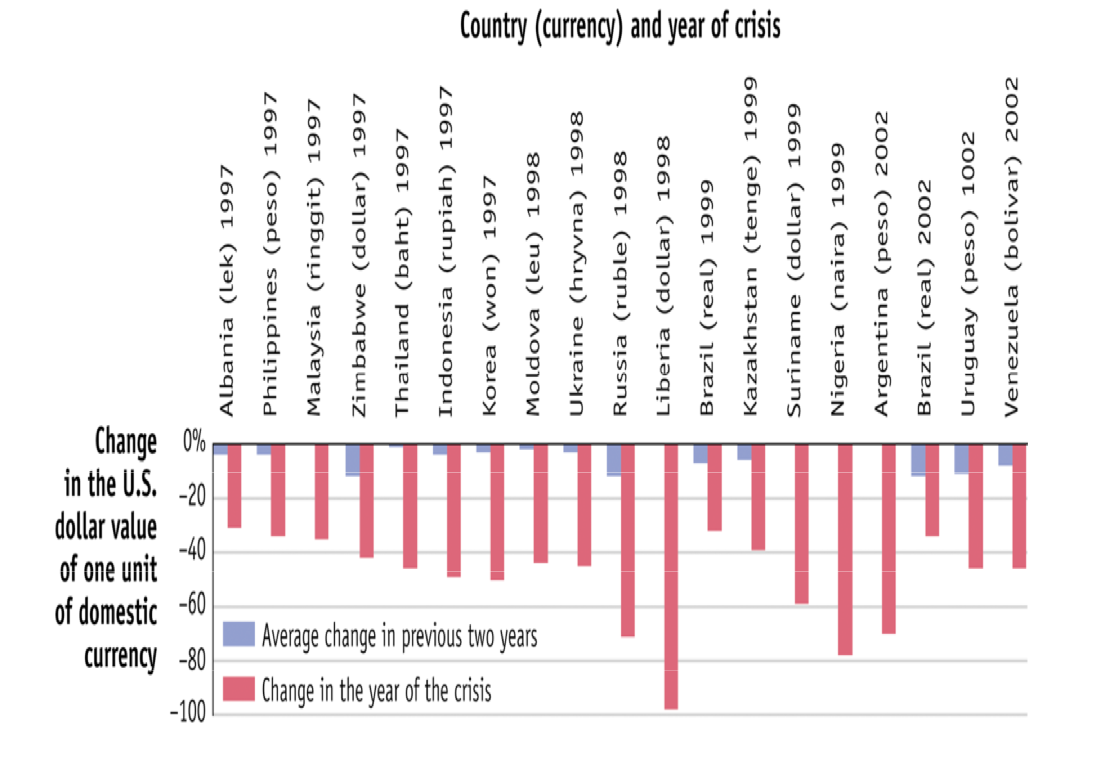
\includegraphics[scale=0.25]{crises.png}
\end{figure}
}

\frame[plain]{
\frametitle{Case Study: Argentina (2001)
}
\begin{itemize}
    \item Depreciated to 70\% in six months!
    \item Effect on importers (good? bad?)
    \item Effect on exporters (good? bad?)
\end{itemize}
\begin{figure}
	\centering
		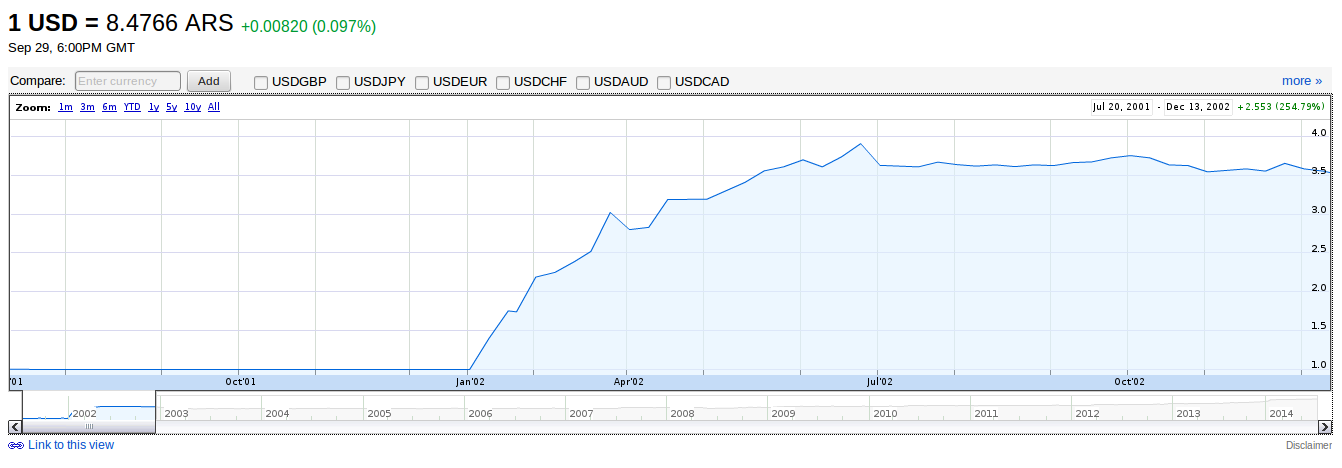
\includegraphics[scale=0.24]{usdars.png}
\end{figure}
}
\begin{frame}{Currency too strong, no worries}
    \begin{itemize}
        \item If depreciation pressure, crisis
        \item If appreciation pressure, no problem
        \item Just accumulate reserves!
    \end{itemize}
    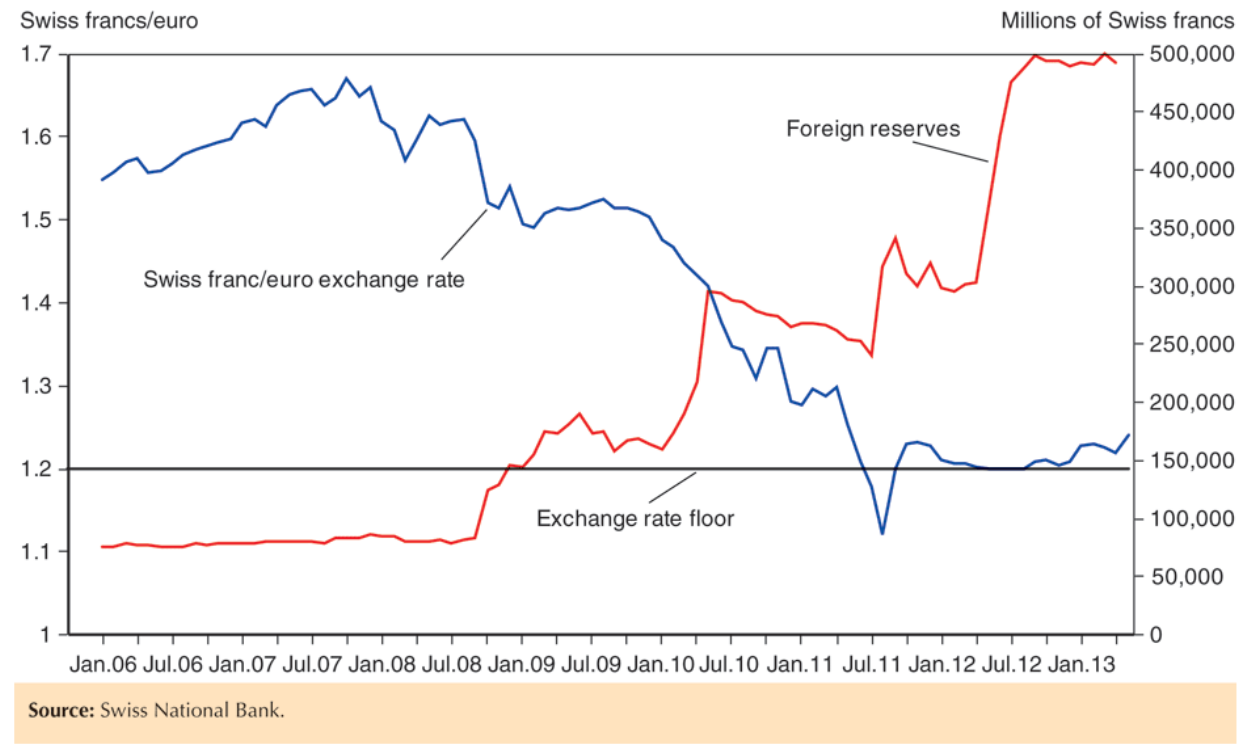
\includegraphics[scale=0.2]{swiss.png}
\end{frame}

\begin{frame}{Pause}
    \begin{itemize}
        \item How does central bank control the exchange rate?
        \item A currency peg ties the central bank's hands
        \item Balance of payments crisis
        \item Next: The puzzle of sterilization
    \end{itemize}
\end{frame}

\begin{frame}{Sterilization}

    \begin{itemize}
        \item Most rich countries manage a float 
        \item Central bank still makes interventions
        \item These are usually \emph{sterilized}
        \item Leave money supply unchanged
        \item Our model: no change in money supply, no change in exchange rate
        \item To explain: add difference in foreign and domestic assets
    \end{itemize}

\end{frame}

\begin{frame}{Parity}

    \begin{itemize}
        \item \emph{perfect asset substitutability:} If investors are indifferent between holding two assets, the two assets are perfect substitutes
        \item We used to call this condition something else\dots
        \item If this condition holds, why buy and sell foreign currency reserves at all?
        \begin{itemize}
            \item Central bank could just sell T-bills to reduce the money supply
            \item Were we being tricky in the balance of payments crisis section? 
        \end{itemize}
    \end{itemize}

\end{frame}

\begin{frame}{Goodbye Parity}

    \begin{itemize}
        \item Until now: assets differ only in expected returns
        \item Add another dimension: risk
        \item Now an investor may be indifferent between: 
        \begin{itemize}
            \item risky asset with high return
            \item safe asset with low return
        \end{itemize}
        \item We no longer have interest rate parity in expected returns! 
        \item \emph{imperfect asset substitutability}
    \end{itemize}

\end{frame}

\frame{
\frametitle{Interest Rate Differentials}
We can consider two different types of risk:
\begin{enumerate}
\item \textbf{Default risk}
\item \textbf{Exchange rate risk}
\end{enumerate}
Interest rate parity
\begin{center}
$  R = R^{*}+ \frac{\left(E^{e} -E\right)}{E}$
\end{center}
can be rewritten as
\begin{center}
$  R = R^{*}+ \frac{\left(E^{e} -E\right)}{E}+\rho$
\end{center}
\begin{center}
$\Rightarrow$ foreign and domestic deposit become imperfect substitutes 
\end{center}
The parameter $\rho$:
\begin{itemize}
\item is the risk premium
\item can be default or exchange risk
\end{itemize}
}

\begin{frame}{Risk premium}

\begin{center}
$  R = R^{*}+ \frac{\left(E^{e} -E\right)}{E}+\rho$
\end{center}

\begin{itemize}
    \item Assume that risk premium increasing function of domestic government bonds held by private sector
    \item Fixing $R^*$ and exchange rates, why does $R$ need to increase if domestic government bonds increase?
    \item Let $B$ be the total amount of government bonds available
    \item Let $A$ be the Central banks holdings of government bonds
    \item We assume that $\rho$ is increasing function of $B-A$ 
\end{itemize}

\end{frame}

\frame[plain]{
\frametitle{Effect of a Sterilized Central Bank Purchase of Foreign Assets Under Imperfect Asset Substitutability}
\begin{figure}
	\centering
		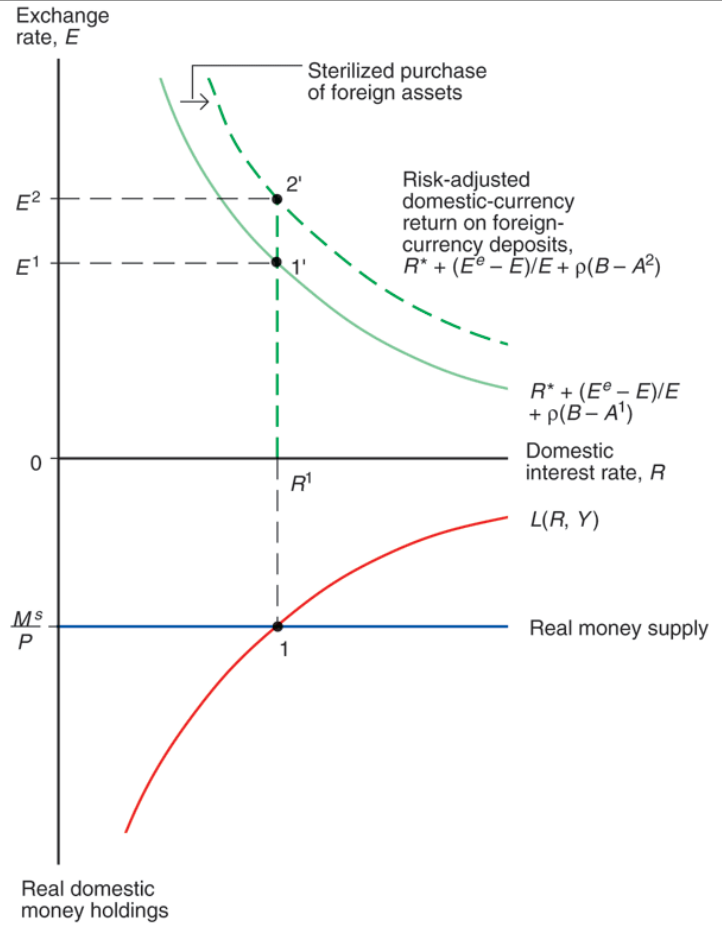
\includegraphics[scale=0.25]{steralized_exchange_rate.png}
\end{figure}
}
  
\begin{frame}{Empirical evidence on sterilized exchange rate interventions}

    \begin{itemize}
        \item No strong evidence that sterilized interventions actually affect exchange rates
        \item However, interest rate parity is violated
        \item May be a signaling effect of government interventions
        \begin{itemize}
            \item Steralized intervention tells market what government is trying to do 
            \item Chandler Lutz researches the effect of government announcements on bond prices 
        \end{itemize}
    \end{itemize}

\end{frame}

\frame{
\frametitle{Types of Fixed Exchange Rate Systems}
\begin{enumerate}
\item\textbf{Reserve currency system:} one currency acts as official international reserves (Bretton Woods, 1944-1973)
\item \textbf{Gold standard:} gold acts as official international reserves that all countries use to make official international payments (1870-1914, 1918-1939)
\item \textbf{Gold exchange standard:} a system of official international reserves in both a group of currencies (with fixed prices of gold) and gold itself.
\item \textbf{Bimetallic standard:} the value of currency is based on both silver and gold.
\end{enumerate}
\begin{itemize}
    \item Talk a little about 1. and 2.
\end{itemize}
}

\begin{frame}{Reserve currency system}
    \begin{itemize}
        \item All countries fix exchange rates to one currency
        \item Implies that all exchange rates are fixed
        \item The country that has the currency is priveleged 
        \begin{itemize}
            \item Prices are normalized, so one currency is free to change real value
            \item This reserve currency can then be used for monetary policy
        \end{itemize}
        \item The unfairness of a dollar reserve currency lead to the end of Bretton Woods
    \end{itemize}
\end{frame}

\begin{frame}{Gold}
    \begin{itemize}
        \item If all currencies fixed to gold, no privelege
        \item Natural limit on monetary policy
        \begin{itemize}
            \item Popular among American fiscal conservatives after 2008
        \end{itemize}
        \item But there are some problems:
        \begin{enumerate}
            \item Gold is commodity money, wasteful 
            \item Monetary policy determined by gold market 
            \item Growing world requires growing gold
            \item Gives power to countries with natural gold resources
        \end{enumerate}
    \end{itemize}
\end{frame}

\frame{% how to print
\frametitle{}
\begin{center}
\textcolor{blue}{Chapter 19. A Short History of the International Monetary System}
\end{center}
}

\frame{
\frametitle{Goals of Macroeconomic Policy}
\textbf{Internal balance}:
\begin{itemize}
\item Full employment of factors 
\item Price level stability
\end{itemize}
\textbf{External balance}
\begin{itemize}
\item Don't borrow too much 
\item Don't lend too much
\end{itemize}
}

\frame{
\frametitle{Goals of Macroeconomic Policies}
Suppose internal balance in the short run occurs when production at potential output or full employment equals aggregate demand:
\begin{center}
$Y_{f} = C\left(Y_{f} - T\right) + I + G + CA\left(\frac{EP^{*}}{P}, Y_{f} - T\right)$
\end{center}
An increase in government purchases (or a decrease in taxes) increases aggregate demand and output above its full employment level.
To restore internal balance in the short run, a revaluation (a fall in E) must occur
}

% \frame{
% \frametitle{Goals of Macroeconomic Policies (3)}
% Suppose external balance in the short run occurs when the current account achieves some value X:
% \begin{center}
% $CA\left(\frac{EP^{*}}{P}, Y �- T\right) = X $
% \end{center}
% An increase in government purchases (or a decrease in taxes) increases aggregate demand, output and income, decreasing the current account.
% To restore external balance in the short run, a devaluation (a rise in E) must occur.            
% }
% 
% \frame[plain]{
% \frametitle{Fig. 19-1: Fig. 19-1: The Policy Trilemma for Open Economies}
% \begin{figure}
% 	\centering
% 		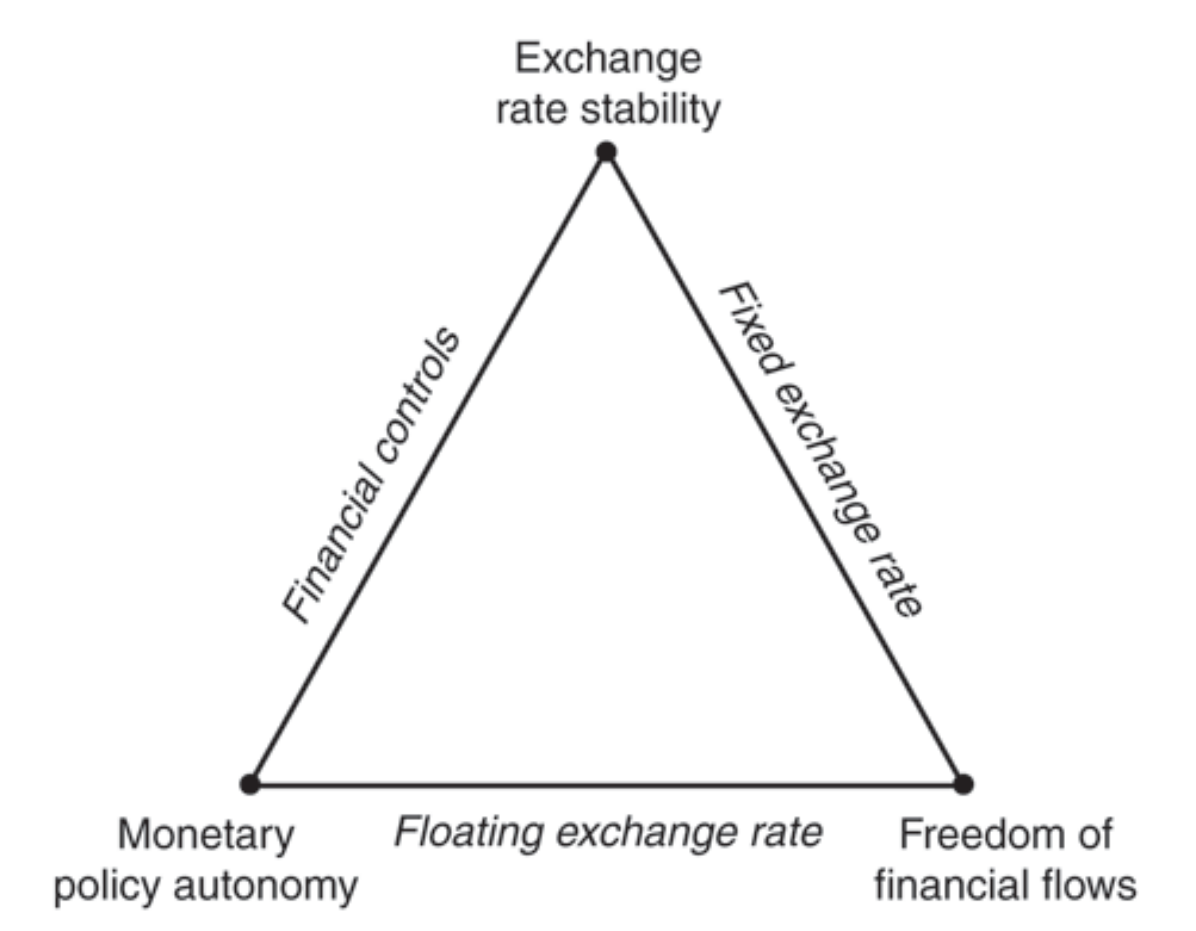
\includegraphics[width=1.00\textwidth]{trilemma.pdf}
% 	\label{fig:11}
% \end{figure}
% }
% 
% 
% \frame[plain]{
% \frametitle{Fig. 19-1: Internal Balance (II), External Balance (XX), and the "Four Zones of Economic Discomfort"}
% \begin{figure}
% 	\centering
% 		\includegraphics[width=1.00\textwidth]{eight.pdf}
% 	\label{fig:11}
% \end{figure}
% }
% 
% \frame[plain]{
% \frametitle{Goals of Macroeconomic Policies (4)}
% \begin{figure}
% 	\centering
% 		\includegraphics[width=1.00\textwidth]{nine.pdf}
% 	\label{fig:11}
% \end{figure}
% }

\end{document}
